%!TEX root = ../dissertation.tex
\begin{savequote}[75mm]
Knowledge knows no bounds.
\qauthor{Creator}
\end{savequote}

\chapter{Motivation for searches beyond the Standard Model}
%\newthought{There's something out there that we don't know.} 

\section{The Standard Model and the Higgs Boson}
\paragraph{}
The Standard Model(SM) is the best description of the microscopic world ~\cite{Griffiths,Tully,Pdg,Schwartz}. 
The SM consists of three generations of leptons ($e$, $\mu$, $\tau$, $\nu_e$, $\nu_{\mu}$, $\nu_{tau}$) and quarks ($u$, $d$, $c$, $s$, $t$, $b$).
They all interact via the weak force. In addition, the charged leptons and quarks interact through the EM force and the quarks also interact through the strong force.
The SM also has the force mediators. EM force mediates through the photon $\gamma$, the strong force meidates through the gluon $g$, and the weak force mediates through $W^{\pm}$ and $Z$ bosons.
The SM predicts everything except the particle's mass, shown in Figure ~\ref{fig:SM}, which are measured experimentally.

\begin{figure}[h!]
  \centering
  \captionsetup{justification=centering}
  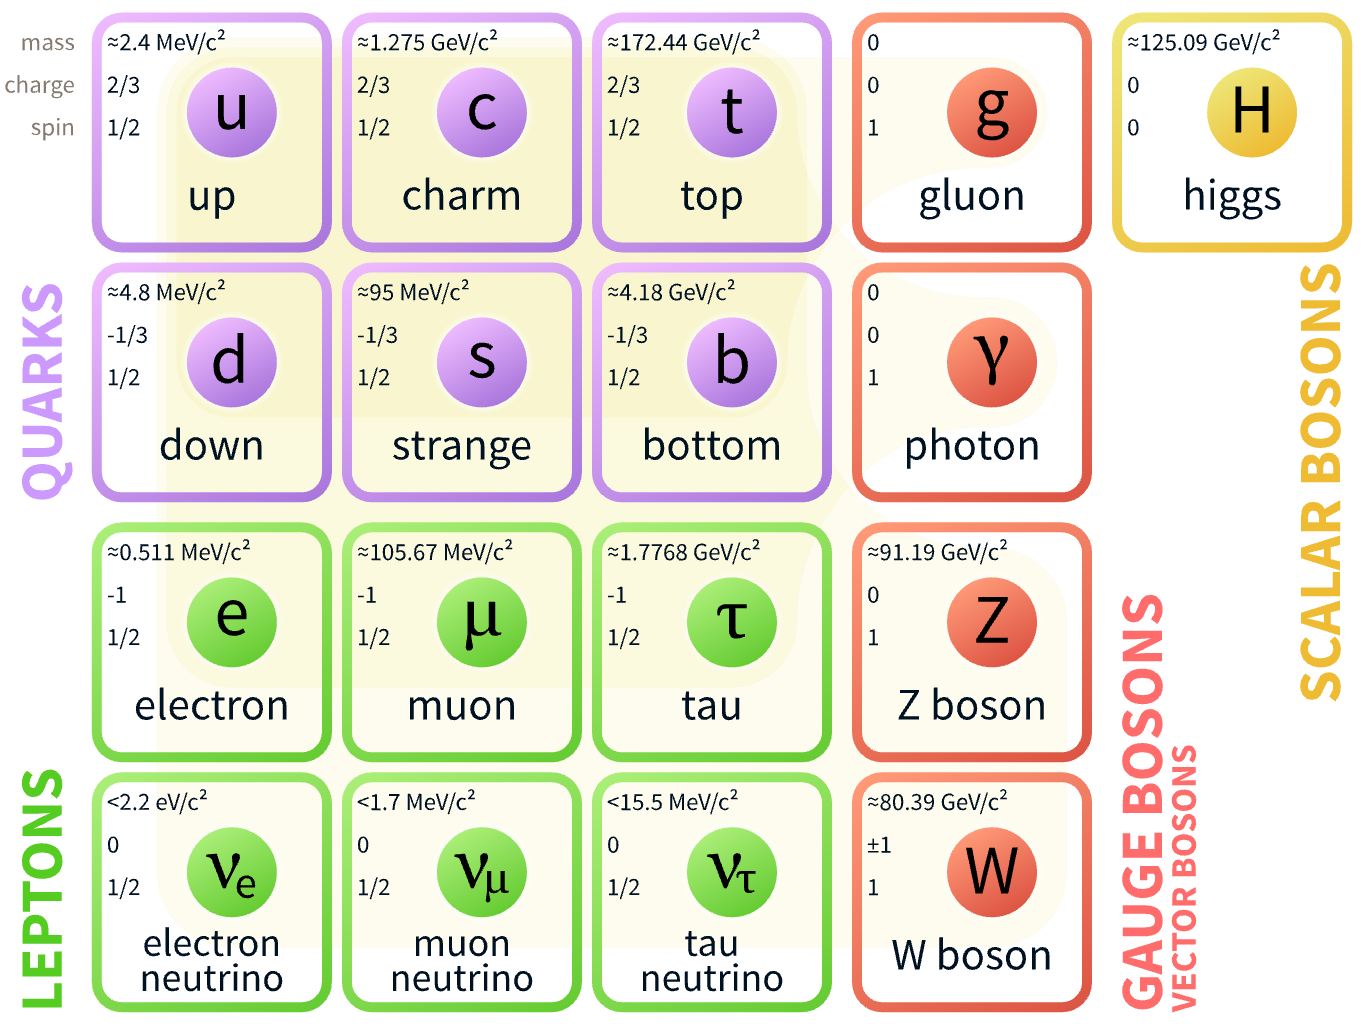
\includegraphics[width=0.6\textwidth]{figures/theory/SM}
  \caption{Fermions and bosons of the Standard Model and their properties~\cite{Pdg}.}
  \label{fig:SM}
\end{figure}

\paragraph{}
However, in SM, due to the gauge invriance under $SU(2)_{L}$, fermions have to be massless in order to have pure left handed states. 
The bosons must also be massless as required by the gauge principle. 
The Higgs mechanism introduces a scalr Higgs field with nonzero vaccum expectation values, which impledes and interacts with the propagation of gague bosons and fermions, hence gives them valid mass terms~\cite{Tully}. 
This broken symmetry of the Standard Model predicts the extra particle degree of freedom as the Higgs boson. The terms inside the Higgs potential are shown in equation~\ref{eqn:higgspotential}.

Include a shape.

\begin{equation}
\label{eqn:higgspotential}
V(\phi_{h}) = \lambda \nu^2 \phi_{h} ^2  + \lambda \nu \phi_{h} ^3  + \frac{1}{4}\lambda \phi_{h} ^4 
\end{equation}

where $\nu$ corresponds to the vaccum expectation value of the field, determined to be around $246$ \GeV.
The first term gives the Higgs mass, $m_h$, as $ \sqrt{2\lambda}\nu$, measured to be $125.09 \pm 0.24$ \GeV. 
The second term provives an $hhh$ vertex, which corresponds to the trilinear coupling of the Higgs boson. 
This means that a two Higgs production (di-Higgs) can happen through a single Higgs even within the Standard Model.

\section{Di-Higgs in the Standard Model}
\paragraph{}
There is much literature about modifications of Higgs self coupling. Using the SM measurements and their precisions, we can constrain the self coupling parameter to an order of magnitude, see \href{https://arxiv.org/abs/1702.07678}{note}.


\section{Di-Higgs in Beyond the Standard Model Physics}


\section{Di-Higgs Decay and search perspectives}

\paragraph{}
Di-Higgs decay is the combination of single Higgs decays. The partile width for Higgs to fermions and bosons (one of them is off-shell) at tree level are shown in equation~\ref{eqn:higgswidth}~\cite{Djouadi}: 

\begin{equation}
\label{eqn:higgswidth}
\begin{array}{cc}
\Tau(h\to f\bar{f} ) = \frac{N_c \sqrt{2} G_{F} m_{f}^2 m_h}{8 \pi} \\
\Tau(h\to VV^{*} ) = \frac{1}{\pi^2} \int_{0}^{M_H^2} \frac{dq_1^2 M_V \Gamma_V}{(q_1^2-M_V^2)^2 + M_V^2\Gamma_V^2} \int_0^{(M_H - q_1)^2} \frac{dq_2^2 M_V \Gamma_V}{(q_2^2-M_V^2)^2 + M_V^2\Gamma_V^2} \frac{\sqrt{2} \delta_v G_{F} m_h^3}{32\pi} \sqrt{\lambda(q_1^2, q_2^2; m_h^2)} [\lambda(q_1^2, q_2^2; m_h^2) + 12\frac{q_1^2q_2^2}{m_h^2}]
%\Tau(h\to WW ) = \frac{2 \sqrt{2} G_{F} m_{W}^2 m_h}{32 \pi} \frac{\sqrt{1 - x_W}}{x_W^2} (3x_W^2 - 4x_w + 4) \\ %only for on shell
%\Tau(h\to ZZ ) = \frac{\sqrt{2} G_{F} m_{z}^2 m_h}{32 \pi} \frac{\sqrt{1 - x_z}}{x_z^2} (3x_z^2 - 4x_z + 4)
\end{array}
\end{equation}
where $N_c$ is the number os colors, $m_f$ is the fermion mass, $G_{F}$ is the Fermi constant. Hence, given the measured Higgs mass, tthe larges brancing ratio is to the \bbbar. Although there is no direct coupling between $h$ and \gg~ at tree level, this decay can happen through W or top loops.

%\paragraph{}CMS latest search result on di-Higgs is also included \href{https://arxiv.org/pdf/1708.08249.pdf}{here}.